\chapter{Introduction}
\label{ch_intro}


Since the discovery of the $\jpsi$ resonance in 1974, the charm energy range (\SIrange{3.0}{4.5}{\GeV}) has been investigated by many experiments in particle physics.
This has led to the further discovery of many more resonances, as shown in \Cref{fig:R_scan}.

\begin{figure}[H]
\centering
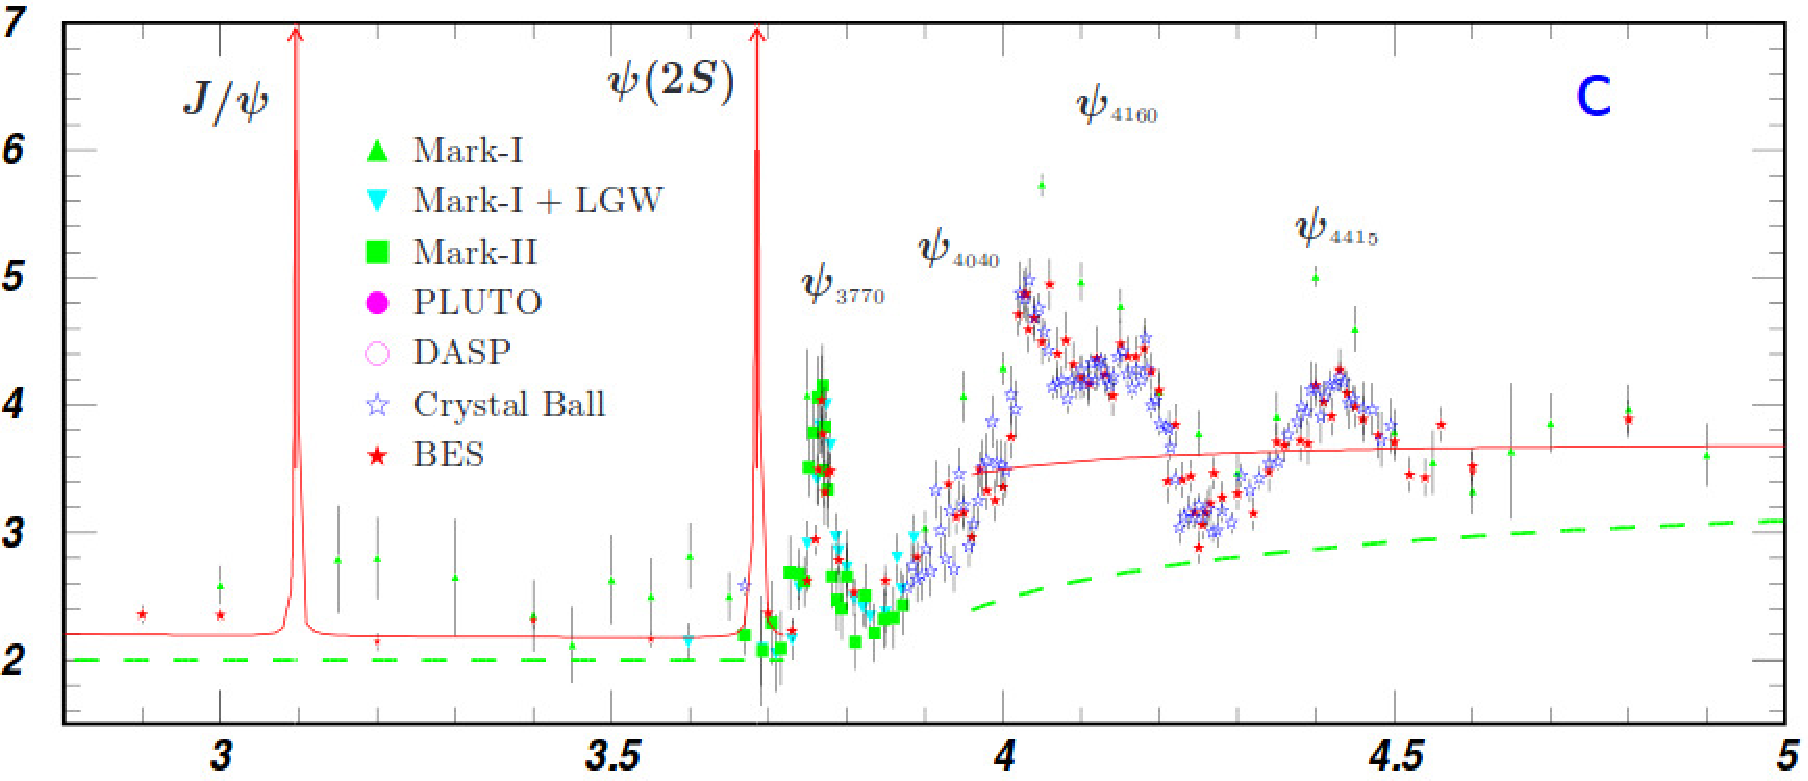
\includegraphics[scale=0.50]{figures/images/R_scan.pdf}
\caption{Measurements of $R = \sigma(\ee \rightarrow \text{(hadrons)}) / \sigma(\ee \rightarrow \mumu)$.}
{Resonances with masses below the $\psipp$ have significantly narrower widths than those above.}
\label{fig:R_scan}
\end{figure}

Many of the lower mass resonances are predictable within the context of the quark model.
However, there are a number of states which have been predicted, but not yet discovered.
There are also states which were discovered experimentally without any corresponding predictions.
A variety of these particles are shown in \Cref{fig:charmonia}.

\begin{figure}[H]
\centering
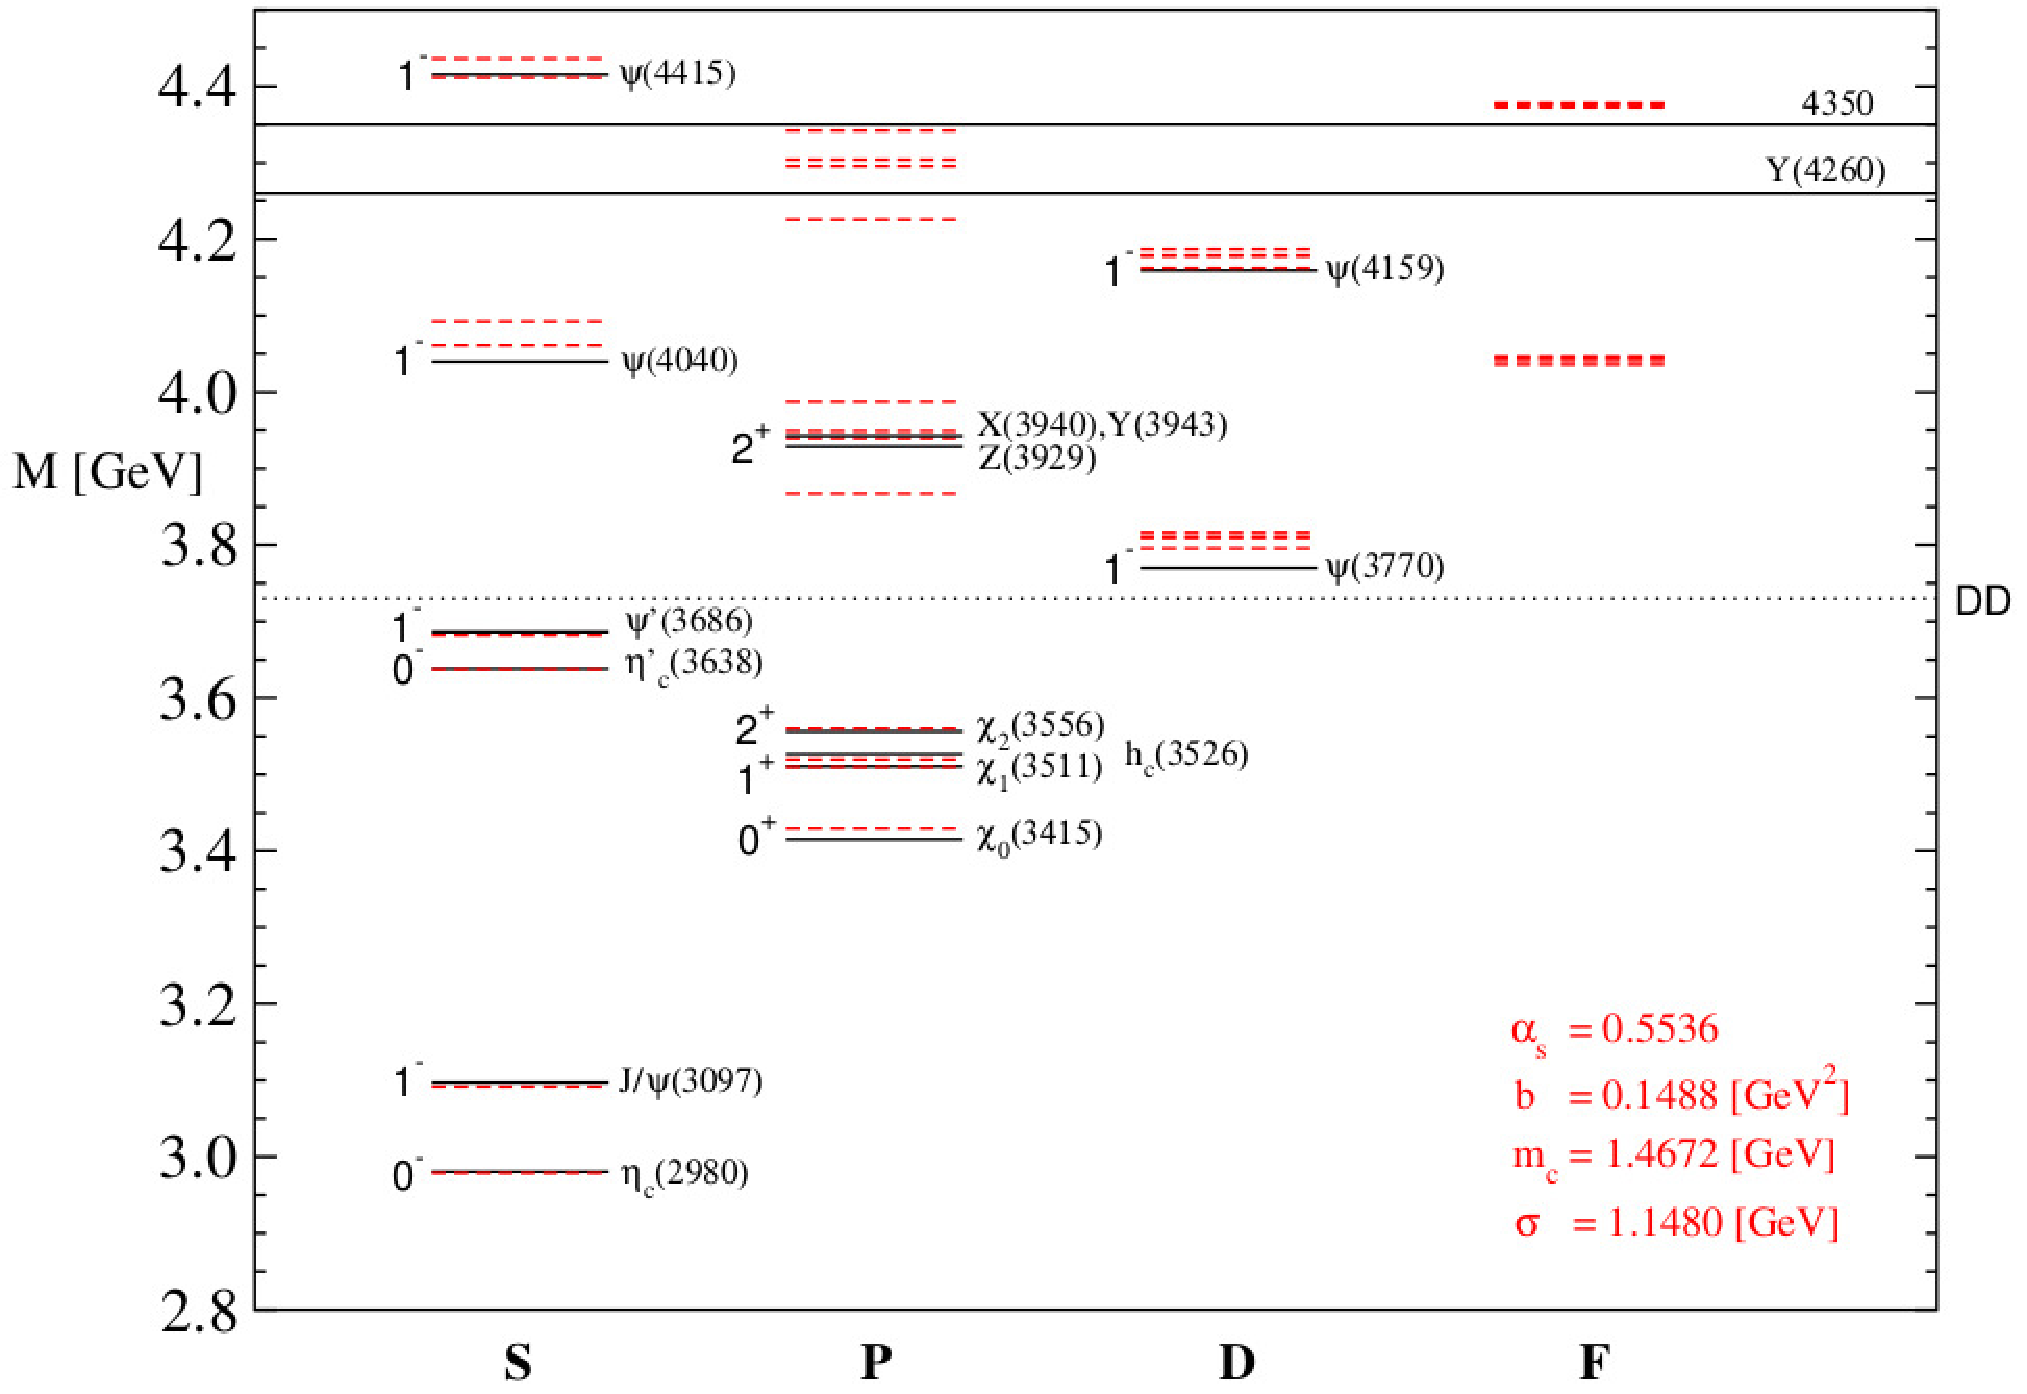
\includegraphics[scale=0.40]{figures/images/charmonia.pdf}
\caption{Measured and predicted charmonium resonances.}
{Many of the measured (black) and predicted (red) values are similar below the $\DDbar$ threshold (dotted line), but show disagreement above this value.}
\label{fig:charmonia}
\end{figure}

The resonances below the $\DDbar$ threshold, like the $\jpsi$ and the $\psip$, show solid agreement with theoretical predictions.
However, many of the ones above, such as the $\psipp$, still show some disagreement.
This is likely due to the more complicated interactions introduced from $\DDbar$ decays.
Several experiments have attempted to measure the shape of the $\psipp$ based on different assumptions.
Many did not account for interference effects, which can notably alter the measured parameters of the $\psipp$, such as the mass, shown in \Cref{tab:previous_results}.

\begin{table}[H]
\centering
\begin{tabular}{c l|c l}
\hline
\multicolumn{2}{c|}{$\Mpsipp$ [\si{\MeV}] (No Interference)} & \multicolumn{2}{c}{$\Mpsipp$ [\si{\MeV}] (With Interference)} \\ [1pt] 
\hline
BES-II \cite{ref:Ablikim:2007}   & 3772.0 $\pm$ 1.9           & BaBar \cite{ref:Aubert:2008b} & 3778.8 $\pm$ 1.9 $\pm$ 0.9 \\
Belle  \cite{ref:Brodzicka:2008} & 3776.0 $\pm$ 5.0 $\pm$ 4.0 & KEDR  \cite{ref:Anashin:2012} & $3779.2^{+1.8 \, +0.5 \, +0.3}_{-1.7 \, -0.7 \, -0.3}$ \\ 
BaBar  \cite{ref:Aubert:2008a}   & 3775.5 $\pm$ 2.4 $\pm$ 0.5 & & \\
\hline
\end{tabular}
\caption{Previous experimental results for the mass of the $\psipp$.}
{Where applicable, the first errors are statistical, the second are systematic, and the third are model-dependent.}
\label{tab:previous_results}
\end{table}

Both BaBar \cite{ref:Aubert:2008b} and KEDR \cite{ref:Anashin:2012} found it necessary to include interference effects in $\DDbar$ production in order to fit to the cross sections of $\ee \rightarrow \gamma\DDbar$ and $\ee \rightarrow \text{(hadrons)}$, respectively.
In the case of the KEDR measurement, the statistics were insufficient to fully resolve the discrepancies seen with other experiments that ignored interference.
{\bf Using the larger data sample available at BESIII, we have precisely measured and analyzed the shape of the $\DDbar$ spectrum around the $\psipp$ resonance.}
We have also used this measurement to probe the branching fraction of $\nonDDbar$ decays in this region.


\section{Procedure}
\label{sec:procedure}

The basis of this measurement involves identifying $\DDbar$ pairs produced in $\psipp$ decays.
All data used in this analysis were collected from $\ee$ collisions analyzed by the BESIII detector.
The $\lel$ and $\alel$ annihilate through a virtual photon, meaning the total energy is transferred to the final state.
Because the input energy can be precisely tuned, specific states with the right quantum numbers, such as the $\psipp$, can be produced.
However, resonances like this will decay almost instantaneously.
For example, the $\psipp$ has an average lifetime of ${\sim}\SI{e-23}{\s}$, and disappears far too quickly to be directly observed.
Even the initial decay into $\DDbar$ pairs is too fast to precisely measure, as the average lifetime ($\tau_{D} \approx \SI{~4e-13}{\s}$) would correspond to a distance of ${\sim}\SI{1}{\mm}$ if it were traveling at $c$.
Because the available energy in these decays is small ($m_{\psipp} - 2 \, m_{D} \approx \SI{40}{\MeV}$), even the maximum velocity ($\beta \approx 0.15$) is too small to observe any displacement in the detector.

% \tau = 1 / 25 [1/MeV] * (200 MeV / 1e-15 m) / (3e8 m / s) = 200 / (3 * 25) e-23 s ~ 10^-13 s

Instead, the reconstruction of candidate $D$ particles relies on measuring their decays into other known modes.
While dozens of decays modes have been measured, we focus on those which have high branching fractions, and are comprised of particles identifiable by the BESIII detector.
For our purposes, these are $\pipm, \Kpm, \piO,$ and $\Ks$.
Each of these particles leaves `tracks' within the detector; charged particles travel along curved paths and interact electromagnetically with charged wires along their trajectory, while neutral particles travel along straight paths and deposit energy in the detector crystals located outside the tracking region.
The various components of the BESIII detector analyze these tracks to determine the type of particle, as well as its momentum and energy.
By analyzing sets of particles corresponding to the chosen decay modes, we can reconstruct the possible combinations and select those most likely to have originated from a $D$ based on their total energy and momentum.


To determine the $\psipptoDDbar$ cross section, we need to count the number of $\DDbar$ pairs produced, as well as measure the total quantity of $\ee$ collisions (the integrated luminosity, $\lum$), at each energy point in our data sample.
This counting is done not only for the actual collision data collected, but also for simulated samples, known as Monte Carlo (MC), to estimate detection efficiencies and backgrounds in our measurement.
Each potential background corresponds to a particular event type which may be mistaken as signal, such as $\ee \rightarrow \tautau$.
We subtract these misidentified contributions from the total amount found in data to determine the actual number of reconstructed $\DDbar$ events.
The detection efficiency of reconstructing $\DDbar$ is determined by counting the number of simulated signal events that pass our selection criteria and dividing by the number of events generated.
Then, using the measured luminosity for each energy point, we determine the cross section as a function of center-of-mass energy ($\Ecm$).


The specific details of this analysis start with Chapter 2, which provides a discussion of relevant theoretical concepts.
Next, Chapter 3 lists the specifications for the collider and detector which collected the data used for these measurements while Chapter 4 describes some of the related analysis software and reconstruction methods. 
From here, Chapter 5 describes the procedure for determining the $\psipptoDDbar$ cross section and shows our measured $\psipp$ parameters with systematic uncertainties.
Finally, Chapter 6 examines the current progress of a related investigation for measuring the $\nonDDbar$ branching fraction of the $\psipp$.

